\documentclass{article}
\usepackage{amsfonts, amsmath, amssymb, amsthm} % Math notations imported
\usepackage{enumitem}
\usepackage[margin=1in]{geometry}
\usepackage{graphicx}
\graphicspath{{./images/}}

\newtheorem{thm}{Theorem}
\newtheorem{prop}[thm]{Proposition}
\newtheorem{cor}[thm]{Corollary}

% title information
\title{Math 181A HW2}
\author{Neo Lee}
\date{04/11/2023}

% main content
\begin{document} 

% placing title information; comment out if using fancyhdr
\maketitle 

\textbf{Problem 1-1}
\begin{enumerate}[label={(3.4.13)}]
    \item 
    For $y \in [0,2]$,
    \begin{align}
        f_Y(y) &= \frac{d}{dy}F_Y(y) \nonumber \\
        f_Y(y) &= \frac{d}{dy}\frac{1}{12}(y^2 + y^3) \nonumber \\
        f_Y(y) &= \frac{1}{12}\left[\frac{y^3}{3}+\frac{y^4}{4}\right] \nonumber \\
        f_Y(y) &= \frac{y^3}{36} + \frac{y^4}{48}. \nonumber 
    \end{align}
\end{enumerate}
\begin{enumerate}[label={(3.4.17)}]
    \item 
    \begin{align}
        P(-a \le Y \le a) & = 1 - P(Y \le -a) - P(Y \ge a) \nonumber \\
        P(-a \le Y \le a) & = 1 - 2P(Y \ge a) \nonumber \qquad (\because P(Y \ge a) = P(Y \le -a)) \\
        P(-a \le Y \le a) & = 1 - 2(1-F_Y(a)) \nonumber \\
        P(-a \le Y \le a) & = 2F_Y(a) - 1. \nonumber
    \end{align}
\end{enumerate}
\begin{enumerate}[label={(3.6.16)}]
    \item 
    \begin{align}
        E\left(\frac{W-\mu}{\sigma}\right) & = E\left(\frac{W}{\sigma}\right) - E\left(\frac{\mu}{\sigma}\right) \nonumber \\
        & = \frac{1}{\sigma}E(W) - \frac{\mu}{\sigma} \nonumber \\
        & = \frac{\mu}{\sigma} - \frac{\mu}{\sigma} \nonumber \\
        & = 0.\nonumber
    \end{align}
    \begin{align}
        Var\left(\frac{W-\mu}{\sigma}\right) & = \frac{1}{\sigma^2} Var(W-\mu) \nonumber \\
        & = \frac{Var(W)}{\sigma^2} \nonumber \\
        & = \frac{\sigma^2}{\sigma^2} \nonumber \\
        & = 1.\nonumber
    \end{align}
\end{enumerate}
\bigbreak

\textbf{Problem 2-1}
For discrete case,
\begin{align}
    E[X] & = \sum\limits_{x \ge a} xP(X=x) + \sum\limits_{x < a} xP(X=x) \nonumber \\
    E[X] & \ge \sum\limits_{x \ge a} aP(X=x) + 0 \nonumber \\
    E[X] & \ge a \sum\limits_{x \ge a}P(X=x) \nonumber \\
    E[X] & \ge a P(X \ge a) \nonumber \\
    P(X\ge a) & \le \frac{E[X]}{a}. \nonumber
\end{align}
It is analogous for continuous case, but just replacing the summation with integral.
\bigbreak

\textbf{Problem 2-2}
Let $\bar{S_n} = \frac{1}{n}\sum\limits_{i=1}^{n}X_i$, and all $X_i$ are i.i.d. Then, 
\begin{align}
    E[\bar{S_n}] & = E[\frac{1}{n}\sum\limits_{i=1}^{n}X_i] \nonumber \\
    E[\bar{S_n}] & = \frac{1}{n}\sum\limits_{i=1}^{n}E[X_i] \nonumber \\
    E[\bar{S_n}] & = \frac{1}{n}nE[X_i] \nonumber \\
    E[\bar{S_n}] & = \mu, \nonumber
\end{align}
and
\begin{align}
    Var(\bar{S_n}) &= Var(\frac{1}{n}\sum\limits_{i=1}^{n}X_i) \nonumber \\
    Var(\bar{S_n}) &= \frac{1}{n^2}Var(\sum\limits_{i=1}^{n}X_i) \nonumber \\
    Var(\bar{S_n}) &= \frac{1}{n^2}\sum\limits_{i=1}^{n}Var(X_i) \nonumber \\
    Var(\bar{S_n}) &= \frac{1}{n^2}nVar(X_i) \nonumber \\
    Var(\bar{S_n}) &= \frac{\sigma^2}{n}. \nonumber
\end{align}
Then, 
\begin{align}
    P(|\bar{S_n} - E[\bar{S_n}]| \ge a) & \le \frac{Var(\bar{S_n})}{a^2} \nonumber \\
    P(|\bar{S_n} - \mu| \ge a) & \le \frac{\sigma^2}{na^2}. \nonumber 
\end{align}
Since $\sigma$ and $a$ are constants, 
\begin{align}
    \lim\limits_{n\rightarrow\infty}P(|\bar{S_n} - \mu| \ge a) & \le 0 \qquad (= 0\because P \ge 0)\nonumber \\
    \lim\limits_{n\rightarrow\infty}P(|\bar{S_n} - \mu| \le a) & = 1. \nonumber
\end{align}
\bigbreak

\textbf{Problem 3-1}
\begin{enumerate}[label={(5.2.23)}]
    \item 
    \begin{align}
        E[X] = \mu & = \sum_{k \in K} kP_X(k;\theta) \nonumber \\
        \mu & = 0 \times \left[\theta^0(1-\theta)^{1-0}\right] + 1 \times \left[\theta^1(1-\theta)^{1-1}\right] \nonumber \\
        \mu & = \theta. \nonumber
    \end{align}

    Then, from the sample, we can estimate 
    \begin{align}
        \hat{\mu} = \frac{1+1}{5} \nonumber \\
        \hat{\mu} = \frac{2}{5} \nonumber \\
        \theta = \mu \approx \hat{\mu}  = \frac{2}{5}.\nonumber \\
    \end{align}
\end{enumerate}
\bigbreak

\textbf{Problem R}
\begin{enumerate}[label=(\arabic*)]
    \item \qquad
    \begin{figure}[h]
        \centering
        \includegraphics*[scale=0.3]{n=10.png}
        \caption{$n=10$}
    \end{figure}

    \item I expect the distribution of the samples would trace closer and closer to a normal distribution, a result directly from Central Limit Theorem. 
    We can see from the plot, the result is what we expected.
    \begin{figure}[h]
        \qquad
        \begin{minipage}{.4\textwidth}
            \centering
            {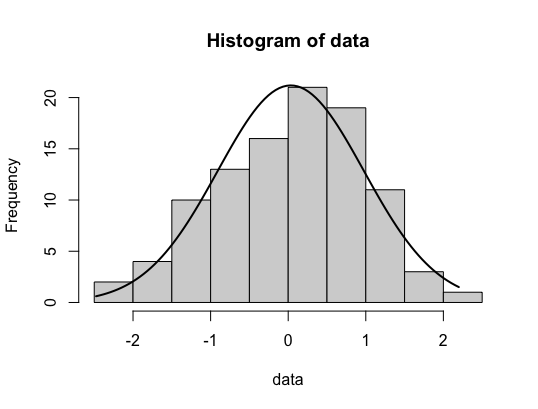
\includegraphics[scale=0.3]{n=100.png}}
            \qquad\qquad$n=100$\label{fig:1}
        \end{minipage}    
        \qquad
        \begin{minipage}{.4\textwidth}
            \centering
            {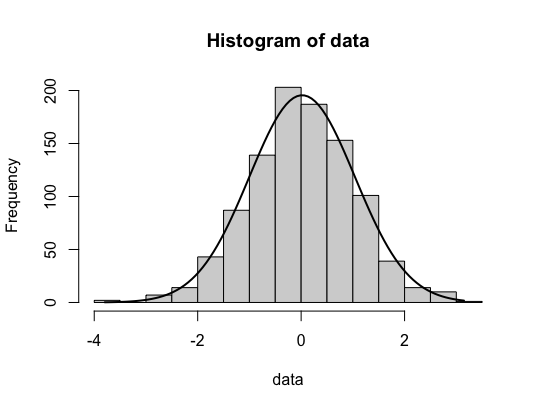
\includegraphics[scale=0.3]{n=1000.png}}
            \qquad\qquad$n=1000$\label{fig:2}
        \end{minipage}   
    \end{figure}
\end{enumerate}

\end{document}